\documentclass{article}
\usepackage{steve}

\lhead{Steve Avery \\ 997694781}
\rhead{ECS 171 - HW 2 \\ \today}

\begin{document}
\section*{Problem 1}

\nblock
Training Weight sample:
\nbstop

\begin{center}
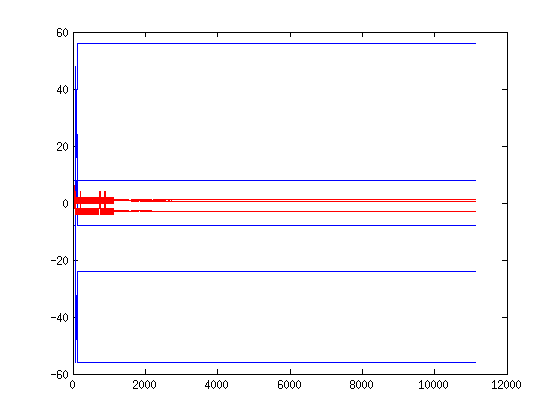
\includegraphics[scale=0.5]{problem1_train.png}
\end{center}

\nblock
This graphic shows the progression of the first output node weights in red,
and the first hidden layer node weights in blue.

Testing Weight sample:
\nbstop

\begin{center}
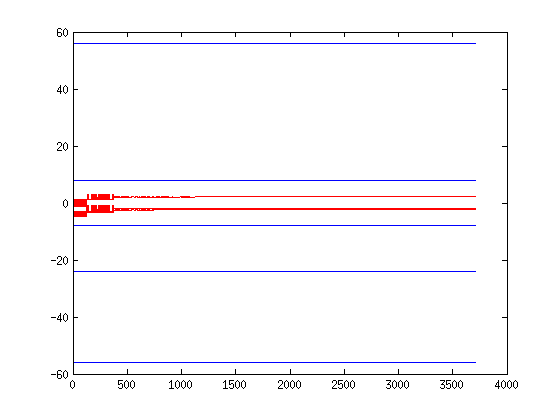
\includegraphics[scale=0.5]{problem1_test.png}

\begin{tabular}{r l l}
Epoch & Training Error & Testing Error \\ 
\hline
1 & 828 & 312 \\
2 & 797 & 307 \\
3 & 797 & 310 \\
4 & 798 & 312 \\
5 & 802 & 309 \\
6 & 802 & 309 \\
7 & 802 & 309 \\
8 & 802 & 309 \\
9 & 802 & 309 \\
10 & 802 & 308
\end{tabular}
\end{center}

\section*{Problem 2}
\nblock
Total training error after 10 epochs is 1038, though I doubt my error values are meaningful.
The activation values are:

\[a_1^{(2)} = g(32 - 16*x_4 - 16*x_5 + 16*x_6 - 16*x_7) \]
\[a_2^{(2)} = g(88.1 - 23.9*x_0 + 7.2*x_1 + 24.8*x_2 + 23.x_3 - 8.1*x_4 - 71.9*x_5 + 23.2*x_6 - 24.8*x_7) \]
\[a_3^{(2)} = g(75.1 - 22.5*x_0 + 39.0*x_1 + 66.3*x_2 + 20.x_3 - 98.3*x_4 - 125.7*x_5 + 84.9*x_6 + 36.9*x_7) \]


\[a_1^{(3)} = g(-.78 - .78*a_1^{(2)} - .78*a_2^{(2)} + 2.3*a_3^{(2)}) \]
\[a_2^{(3)} = g(-1.89 - 1.89*a_1^{(2)} + 2.11*a_2^{(2)} + 1.67*a_3^{(2)}) \]
\[a_3^{(3)} = g(0) \]
\[a_4^{(3)} = g(-2.33 + 1.67*a_1^{(2)} + 1.67*a_2^{(2)} - a_3^{(2)}) \]
\[a_5^{(3)} = g(0) \]
\[a_6^{(3)} = g(-3 + a_1^{(2)} + a_2^{(2)} + a_3^{(2)}) \]
\[a_7^{(3)} = g(0) \]
\[a_8^{(3)} = g(0) \]
\[a_9^{(3)} = g(.78 + .78*a_1^{(2)} - 2.78*a_2^{(2)} + 1.22*a_3^{(2)}) \]
\[a_{10}^{(3)} = g(0) \]

\nbstop

\section*{Problem 3}
\nblock
After forward propagation the activation of each node have these values:

\begin{tabular}{c c c c c c c c c c}
1 & 1 & -1 & -1 & -1 & -1 & -1 & -1 & & \\
-1 & -1 & -1 & & & & & & & \\
-1 & -1 & -1 & -1 & -1 & -1 & -1 & -1 & -1 & -1
\end{tabular}

The weights are initialized at zero, so the fact that none of the nodes beyond 
the input layer activated makes sense.

The expected value of the selected sample was MIT, which would have 
looked like this output vector:

\begin{tabular}{c c c c c c c c c c}
-1 & -1 & 1 & -1 & -1 & -1 & -1 & -1 & -1 & -1
\end{tabular}

Which makes the output error

\begin{tabular}{c c c c c c c c c c}
0 & 0 & 2 & 0 & 0 & 0 & 0 & 0 & 0 & 0
\end{tabular}

Now we can calculate the error for the hidden layer.
First we need to get the weights connecting the first node
of the hidden layer to each node of the output layer.
Since all of the weights for the first round are at zero,
this vector is 10 zeros.

This implies that the error on each node in the hidden layer will 
be zero because multiplying by the all zero vectors will result in 
zeros.

So the total error for all nodes:

\begin{tabular}{c c c c c c c c c c}
- & - & - & - & - & - & - & - & & \\
0 & 0 & 0 & & & & & & & \\
0 & 0 & 2 & 0 & 0 & 0 & 0 & 0 & 0 & 0
\end{tabular}

Now we can use the errors to update the weights. We iterate in reverse through
the layers of the neural network. The first two nodes will not update their weights
because they had zero error for this round.

Update the weight on the bias term for the third node:
\[\alpha = 1\]
\[w = 0 + \alpha * \delta = 2\]

Updating the weights on the input from each hidden layer node:
\[w = 0 + \alpha * \delta * -1 = -2\]

$\delta$ is the error for this node, and it has value 2. The activation of all
nodes previous to this layer is -1. So the final weight for this node will be:
\[a_3^{(3)} = g(2 - 2*a_1^{(2)} - 2*a_2^{(2)} - 2*a_3^{(2)}) \]

No other node will update this round. This agrees with the code I wrote:
\nbstop

\begin{center}
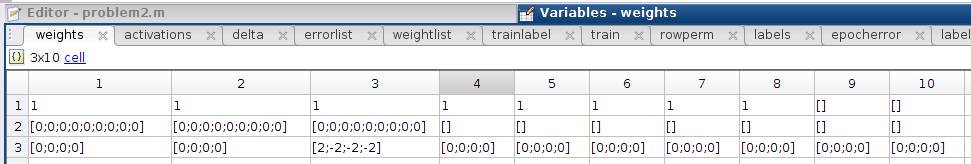
\includegraphics[scale=0.5]{scr.png}
\end{center}


\section*{Problem 4}
The lowest testing error is from 2 hidden layers of 8 nodes each. But this could be overfitting.

\begin{tabular}{r l l l l}
Hidden Layers & 3 nodes per layer & 5 nodes per layer & 8 nodes per layer & 10 nodes per layer \\
\hline
1 & 321.33 & 321.24 & 343.37 & 315.12 \\
2 & 352.24 & 332.87 & 311.04 & 316.43 \\
3 & 314.97 & 316.42 & 321.06 & 340.78
\end{tabular}

\section*{Problem 5}
\nblock
My classifier puts this sample in the CYT category.
\nbstop

\end{document}
